%In the fast-evolving landscape of healthcare, seamless collaboration between multiple organizations is essential to ensure the highest standard of patient care. We delve into the application of Trusted Execution Environment (TEE) to facilitate the secure exchange of event logs between three pivotal actors: an esteemed hospital, a specialized clinic, and a leading pharmaceutical company. This innovative approach fosters a robust and trustworthy ecosystem where sensitive patient data can be shared securely, promoting seamless collaboration for the betterment of patient outcomes.

%Sintetizza il processo tra ospedale azienda farmaceutica e struttura specializzata
In the medical field, cooperation between the various structures is crucial, and many processes are outsourced. 
When a patient enters the hospital, preliminary examinations are carried out and then the hospital company orders from the pharmaceutical company the drugs needed to treat the patient. The pharmaceutical company receives the order and if the drugs is not available, prepares it in the laboratory, otherwise sends it to the requesting hospital. The hospital will manage the drugs received and check whether the patient can be treated in hospital or not. If the patient requires special care, the patients will be transferred to a specialised clinic where more in-depth checks will be carried out. If necessary, the specialised clinic will order drugs from the pharmaceutical company, which will supply them, depending on availability. Once the response to the alternative treatment has been verified, the patient is transferred back to the hospital to prepare for dehospitalisation. Before discharging the patient, the hospital prepares the necessary clinical documentation in order to discharge the patient. it also carries out analysis checks and then declares the patient cured to be discharged.
%Storiella sullo scambio e utilizzo dei dati

As the hospital is in cooperation with the specialised clinic and the pharmaceutical company, it is decided one day to analyse the entire process by considering data from all three partners to provide an overview of the process. The hospital makes a request for the necessary data from all companies participating in the co-operation. All companies will proceed with sending their process data in the form of event logs and in order to mine all data together, the hospital must merge the event logs. Once the event log has been merged, the hospital can proceed with the execution of the mining algorithm to analyse the entire process.


\begin{figure}[t]
\centering
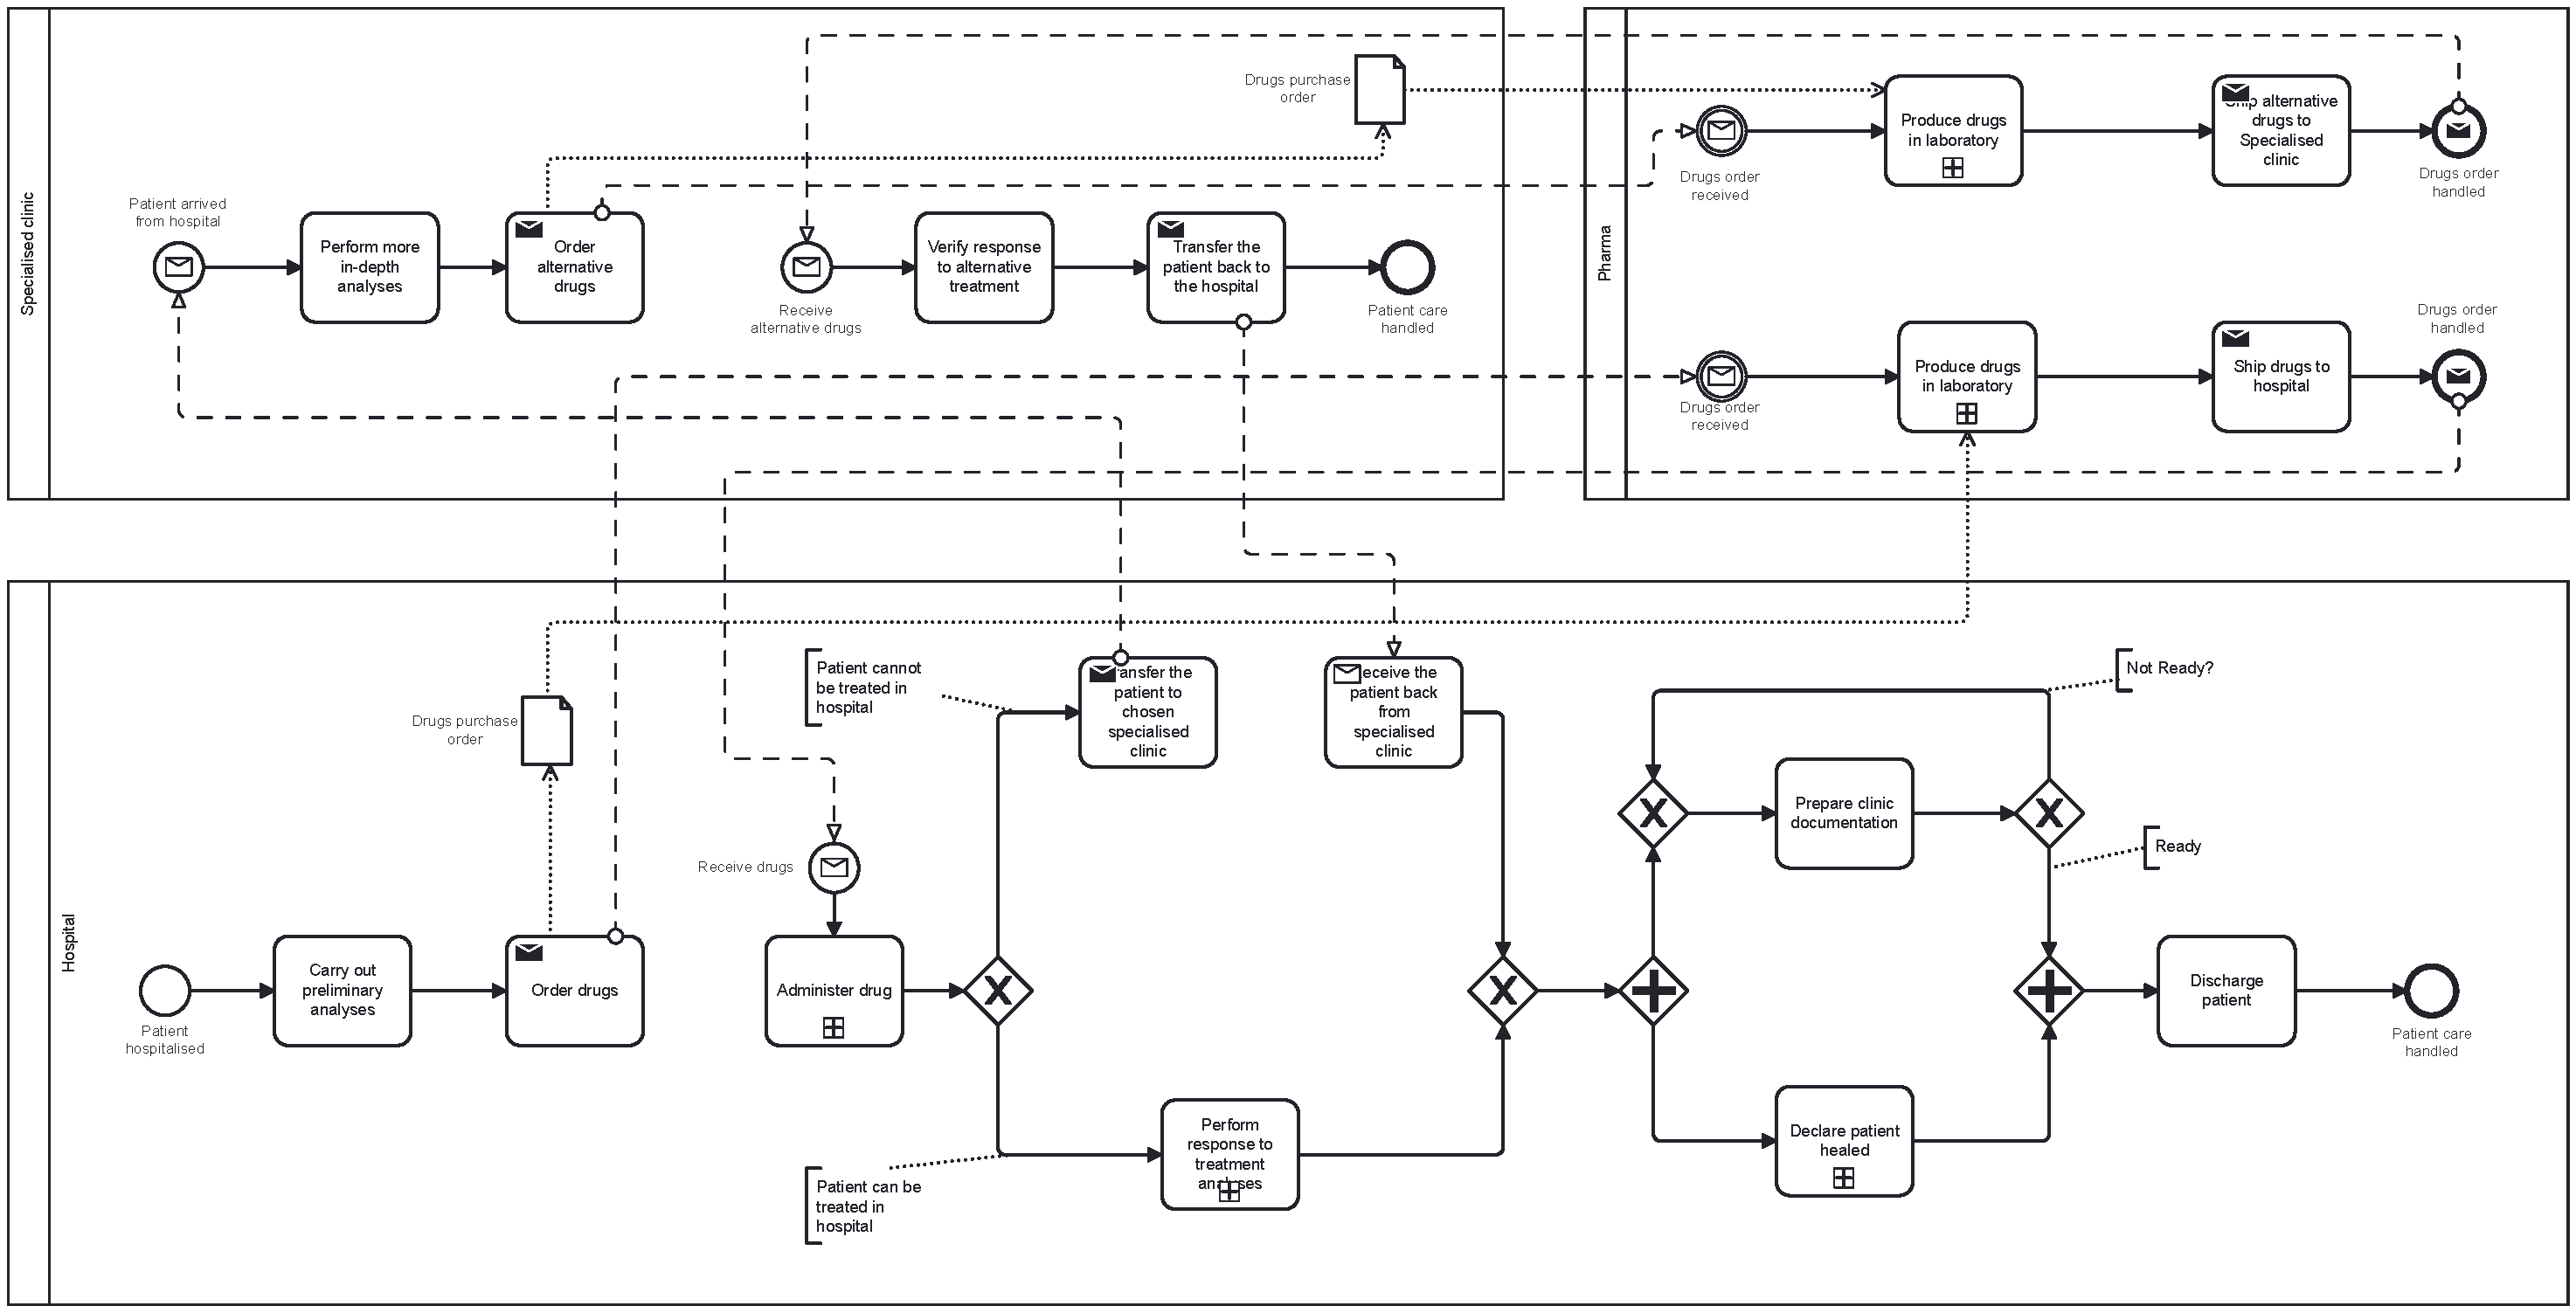
\includegraphics[width=10.5cm]{content/figures/healthcare_scenario.pdf}
\caption{BPMN Healthcare Scenario}
\label{fig:sequence_diagram}
\end{figure}